\section{Methods}



\subsection{Aggregation}



\subsection{Beta Algorithm}
\begin{figure}[H]
\caption{Pseudo-code for Beta algorithm \cite{Nembrini2002}}
\begin{lstlisting}
Create list of neighbours for robot, Nlist
k = number of neighbours in Nlist
i = 0

loop forever {
	i = i modulo cadence

	if (i = 0) {
		Send ID message

		Save copy of k in LastK
		Set reaction indicator Back to FALSE
		k = number of neighbours in Nlist
		Create LostList comparing Nlist and OldList

		for (each robot in LostList) {
			Find nShared, number of shared neighbours
			if (nShared <= beta) {
				Set reaction indicator Back to TRUE
			}
		}

		if (Back = TRUE) {
			turn robot through 180 degrees
		}
		else if (k > LastK) {
			make random turn
		}
		
		Save copy of Nlist in Oldlist
	}
	Steer the robot according to state
	Listen for calls from robots in range
	Grow Nlist with neighbours IDs and connection info

	i++
}
\end{lstlisting}
\label{fig:pseudocode}
\end{figure}


\subsection{Movement}



\subsection{Connection}



\subsection{System variables}



\subsection{Automaton}
\begin{figure}[H]
\caption{Timed automaton for the Beta algorithm}
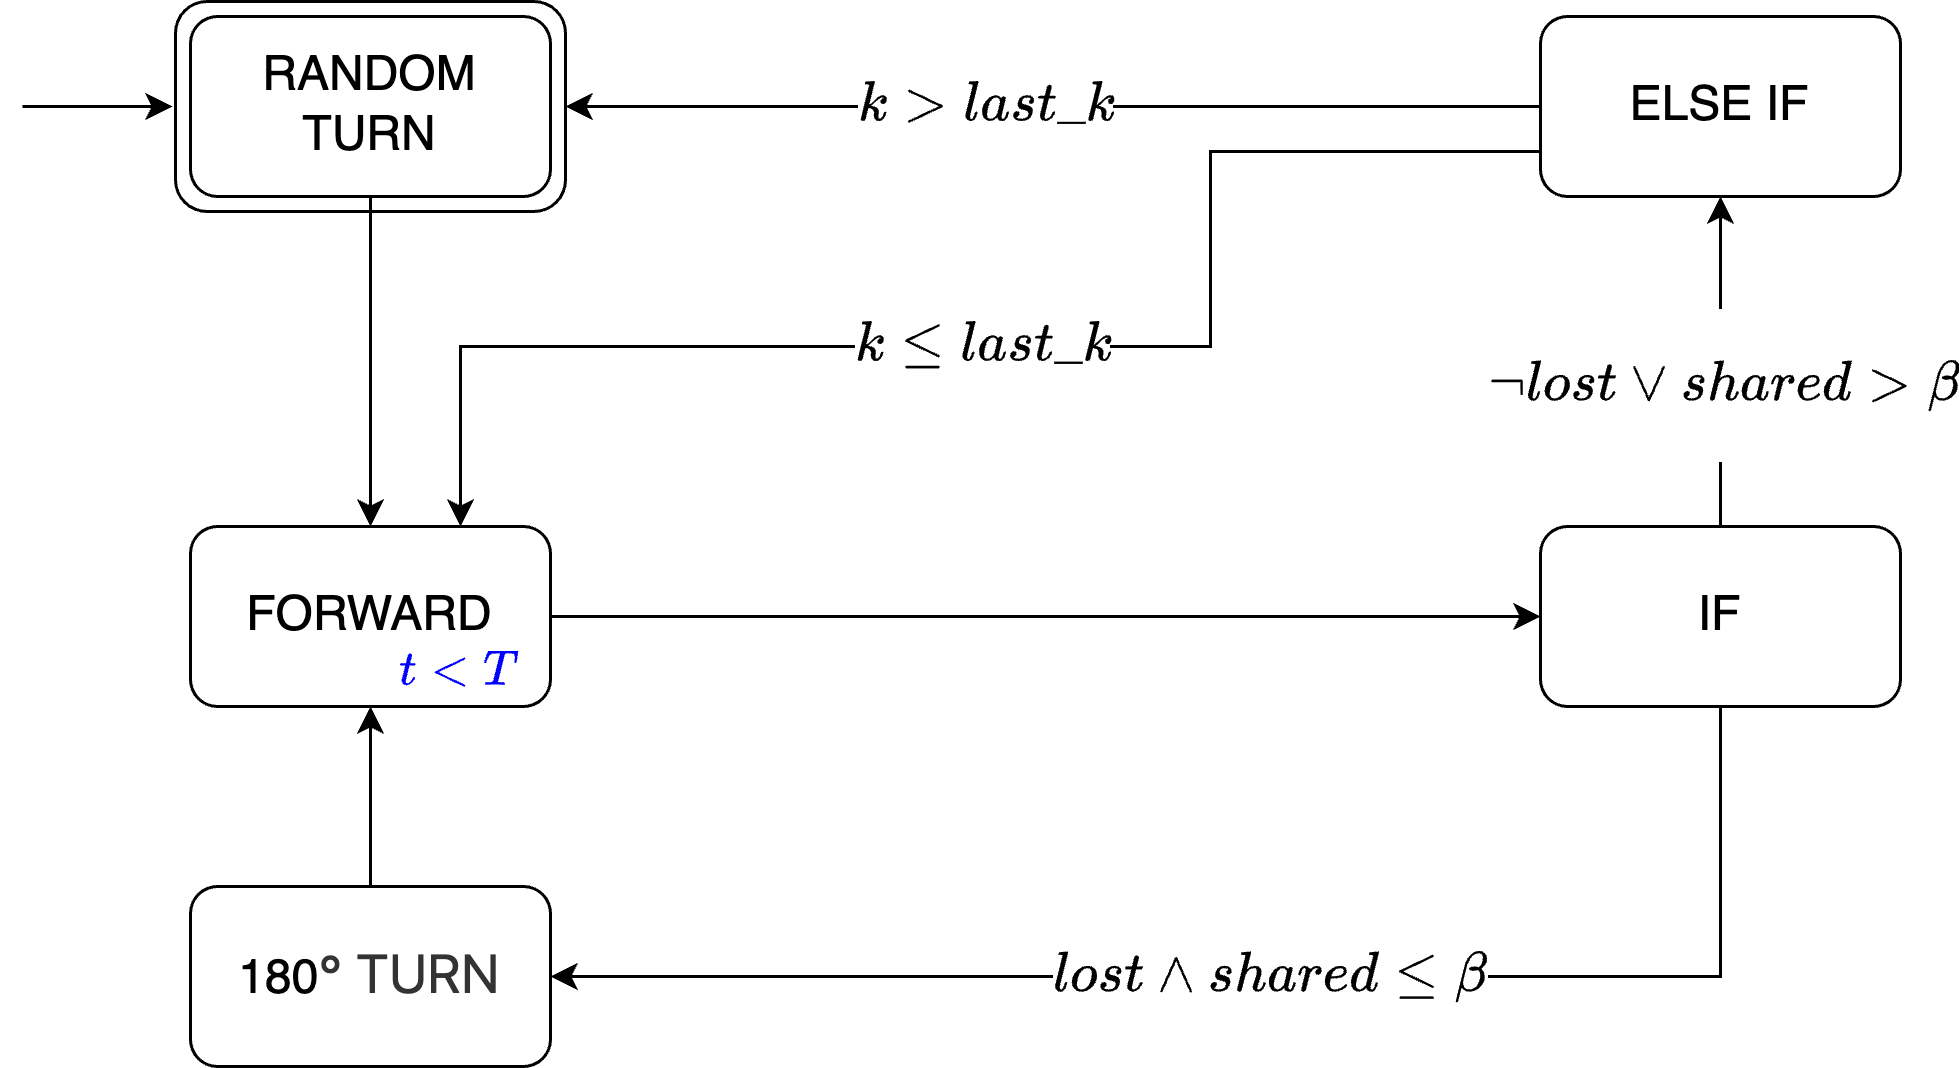
\includegraphics[width=\textwidth]{images/beta.png}
\label{fig:automaton}
\end{figure}
